\icode{E-MD-SI-L2-261115-001}
如图所示，升降机内的水平地板上，用轻弹簧连接一个的物体，弹簧处于拉伸状态，当升降机以速度 \(v\) 向下做匀速运动时，物体恰好能静止在地板上，若突然发现物体在升降机内向右运动，则升降机的运动情况可能是\paren[]
	
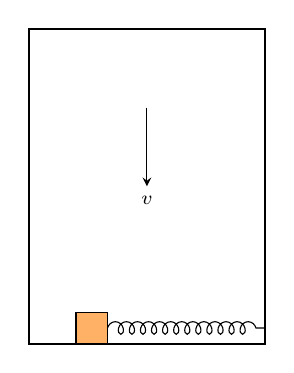
\begin{tikzpicture}[font=\scriptsize]
	\draw[thick] (0,0) rectangle(3,4);
	\draw[fill=orange!60] (.6,0) rectangle(1,.4);
	\draw[decoration={aspect=.8,segment length=4,amplitude=.8mm,coil},decorate] (1,.2)--(3,.2);
	\draw[-stealth] (1.5,3)--(1.5,2)node[below]{\(v\)};
\end{tikzpicture}
\begin{choices}
	\item 保持原来匀速运动
	\item 向下做加速运动
	\item 向下做减速运动
	\item 已停止不动
\end{choices}
\begin{answer}
    B\qquad 提示：
\end{answer}